% DO NOT COMPILE THIS FILE DIRECTLY!
% This is included by the other .tex files.

\begin{frame}[t,plain]
\titlepage
\end{frame}

\section{MISP}

\begin{frame}
\frametitle{What is MISP?}
\begin{itemize}
       \item MISP is an OSS {\bf threat information sharing} platform (TISP)
       \item A tool used and deployed by CSIRTs, SOCs, Cyber threat researchers around the world
       \item The main objective is {\bf collective defense} against threats
\end{itemize}
\end{frame}

\begin{frame}
 \frametitle{MISP: Started from a practical use-case}
 \begin{itemize}
         \item During a malware analysis workgroup in 2012, we discovered that we worked on the analysis of the same malware.
         \item We wanted to share information in an easy and automated way {\bf to avoid duplication of work}.
         \item Christophe Vandeplas (then working at the CERT for the Belgian MoD) showed us his work on a platform that later became MISP.
         \item A first version of the MISP Platform was used by the MALWG and {\bf the increasing feedback of users} helped us to build an improved platform.
         \item MISP is now {\bf a community-driven development} supporting different intelligence communities.
 \end{itemize}
\end{frame}

\begin{frame}
\frametitle{Development based on practical user feedback}
\begin{itemize}
    \item Organic growth over time within security teams:
        \begin{itemize}
                \item {\bf Malware reversers}: share indicators of analysis with colleagues.
                \item {\bf Security analysts} searching, validating and using indicators in ops.
                \item {\bf Intelligence analysts} researching adversary groups.
                \item {\bf Risk analysis teams} monitoring trends, threats, remediations.
        \end{itemize}
    \item Some examples of other communities picking up MISP:
        \begin{itemize}
                \item {\bf Financial sector}: sharing financial indicators, fraud information.
                \item {\bf Law-enforcement}: bootstrapping DFIR cases, non-cyber-threats, border control, etc
                \item {\bf Military} sharing highly specialised information.
                \item {\bf Disinformation research}: Election interference, disinfo campaigns, etc.
        \end{itemize}
\end{itemize}
\end{frame}

\begin{frame}
\frametitle{Objectives of MISP in more detail}      
\begin{itemize}
       \item A tool that {\bf collects threat information} from partners, your analysts, your tools, sensors, feeds
       \item Normalises, {\bf correlates}, {\bf enriches} the data
       \item Manages your processes and automates tasks such as {\bf notifications}, {\bf data flow management}, {\bf triaging} and so on
       \item Allows teams and communities to {\bf collaborate} and rapidly {\bf exchange knowledge}
       \item {\bf Feeds} automated protective tools and analyst tools with the output
       \item {\bf Presents} both individualised and community centric facts, trends, reports of the intelligence
\end{itemize}
\end{frame}

\begin{frame}
\frametitle{A bit more details about the MISP software}      
\begin{itemize}
       \item {\bf OSS}, hosted on github with a very active developer and user community behind it
       \item Users can either: 
       \begin{itemize}
           \item {\bf deploy their own MISPs}
           \item {\bf Join an existing MISP instance} hosted by someone else
       \end{itemize}
       \item MISP instances can be {\bf interconnected}, creating networks with different topologies (mesh, hub/spoke, hybrid)
\end{itemize}
\end{frame}

\begin{frame}
    \frametitle{Typical interconnection scenario}
    \begin{center}
        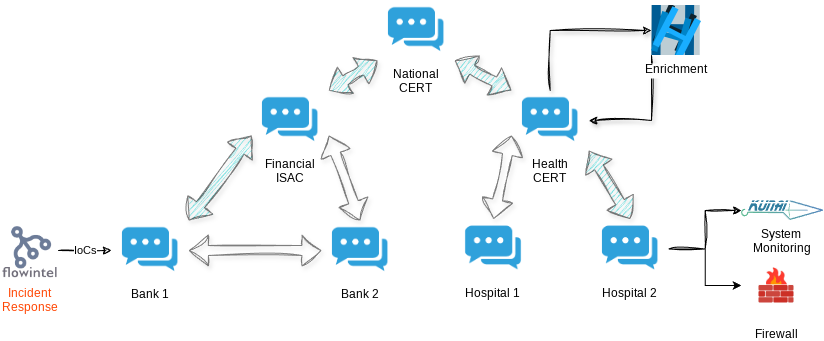
\includegraphics[width=1\linewidth]{MISP_community.png}
    \end{center}   
\end{frame}

\begin{frame}
\frametitle{What is the MISP-project?}
\begin{itemize}
        \item Besides being a a web application, the MISP-project also contains the following:
        \begin{itemize}
            \item A set of {\bf open standards} (implemented by MISP and other tools)
            \item An {\bf ecosystem} of libraries, supporting tools
            \item A collection of guidance and best practice documentation by practitioners
        \end{itemize}
        \item All of these are free \& open source
\end{itemize}
\end{frame}

\begin{frame}
    \frametitle{Information pipeline}
    \begin{center}
        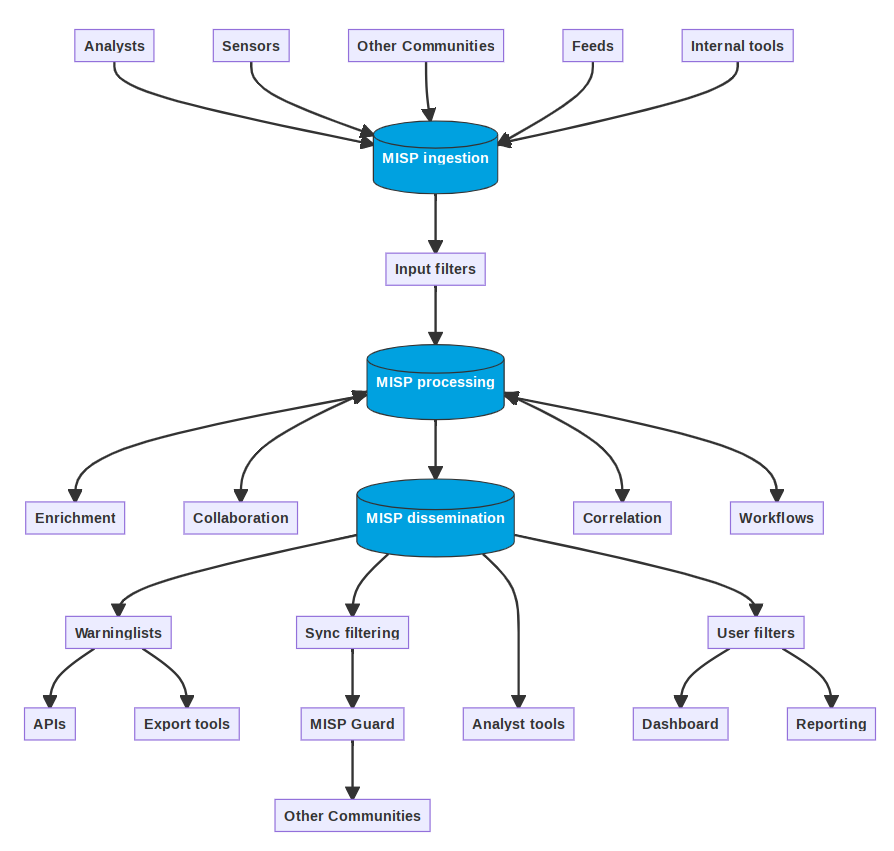
\includegraphics[width=0.75\linewidth]{misp_data_flow.png}
    \end{center}
\end{frame}


\section{How can this be relevant to you?}

\begin{frame}
\frametitle{Why should you care?}
    \begin{itemize}
        \item You're looking to improve your security posture
        \begin{itemize}
            \item If you have a {\bf security team / operations team} looking for threat intel
            \item If you would like to {\bf automate} your security processes
            \item If you are dealing with security {\bf incidents} and would like to {\bf collaborate}
        \end{itemize}
        \item If you're looking for ways to overcome internal challenges
        \begin{itemize}
            \item We've been building this by now rather complex application since 2012
            \item Long list of {\bf libraries, techniques, ideas} that can be reused
            \item Well established standards for information exchange
            \item Can be adapted to completely {\bf different sharing use-cases} you may have
        \end{itemize}
    \end{itemize}
\end{frame}

\begin{frame}
\frametitle{Why rely on MISP, an open source platform for all of this?}
    \begin{itemize}
        \item Extremely mature and actively maintained
        \item Continuously vetted 
        \begin{itemize}
            \item Regular {\bf penetration tests} by multiple parties
            \item Actively {\bf used across most sectors worldwide}, including military, governmental, private sector, NGOs, etc
            \item Run by a {\bf CERT}: Open policy on {\bf vulnerability handling policy}, security is the top priority at all times
        \end{itemize}
    \end{itemize}
\end{frame}

\begin{frame}
\frametitle{Why rely on MISP, an open source platform for all of this?}
    \begin{itemize}
        \item We build our software with an {\bf open source mindset}
        \item Make the tool fit your workflows, modify what you don't like
        \begin{itemize}
            \item We also make it a priority to {\bf incorporate code contributions} (after thorough analysis)
            \item Provided are {\bf tooling, GUI based systems, plug-in systems and extensive APIs} for customisation
            \item Guides, training materials, documentation to achieve the above
        \end{itemize}
    \end{itemize}
\end{frame}

\begin{frame}
\frametitle{Why rely on MISP, an open source platform for all of this?}
    \begin{itemize}
        \item {\bf Every cent of your TIP budget goes to what really matters}:
        \begin{itemize}
            \item Building {\bf competency} within your team
            \item {\bf Infrastructure} for running MISP and other tooling
        \end{itemize}
        \item Interoperability
        \begin{itemize}
            \item {\bf Open standards}, support for a long list of other formats
            \item Our {\bf objective isn't to lock you into a walled garden}
        \end{itemize}
    \end{itemize}
\end{frame}


\begin{frame}
\frametitle{Why do we develop all of this?}      
\begin{itemize}
   \item {\bf Main goal}: Make our own lives and the lives of our constituency easier
   \begin{itemize}
       \item Our central tool for ingesting, storing and disseminating information...
       \item ...as well as to interact with organisations
       \item By solving issues of other communities, we already have them prepared for information sharing with us when needed
   \end{itemize}
   \item {\bf Secondary}: Democratise threat intelligence for all
   \item {\bf Stretch goal}: Build a full open-source tool-chain for CSIRTs / SoCs / etc
\end{itemize}
\end{frame}

\section{To wrap it up...}

\begin{frame}
\frametitle{How to get involved?}      
\begin{itemize}
   \item Simply {\bf use the tool} and give us feedback of what works or doesn't work for you
   \item Get active in the {\bf MISP OSS community}
   \item Join one, or {\bf start your own sharing community}!
   \item Join the {\bf private sector MISP community hosted by CIRCL} to exchange threat intel with a massive community
   \item Join us at \url{https://hack.lu}
\end{itemize}
\end{frame}


\begin{frame}
  \frametitle{Get in touch if you have any questions}
  \begin{itemize}
    \item Contact me:
    \begin{itemize}
      \item andras.iklody@circl.lu \url{https://twitter.com/iglocska} \url{https://infosec.exchange/@iglocska}
    \end{itemize}    
    \item Contact us:
    \begin{itemize}
      \item info@circl.lu \url{https://twitter.com/circl_lu} \url{https://www.circl.lu/}
      \item \url{https://github.com/MISP} \url{https://www.misp-project.org/}
      \item \url{https://twitter.com/MISPProject} \url{https://misp-community.org/@misp}
      \item \url{https://github.com/cerebrate-project} \url{https://www.cerebrate-project.org/}
    \end{itemize}
  \end{itemize}
\end{frame}

